\documentclass[a4paper,12pt]{report}

\usepackage[utf8]{inputenc}
\usepackage{graphicx}
\usepackage{helvet}
\usepackage[italian]{babel}
\usepackage{amsthm}
\usepackage{hyperref}

\newtheorem{enunciato}{Enunciato}

\begin{document}
\begin{titlepage}
    \centering
    
\includegraphics[width=0.5\textwidth]{img/logo.png}\par\vspace{1cm}
    {\scshape\Large Corso di Laurea in Ingegneria e Scienze Informatiche\par}
    \vspace{1.5cm}
    {\huge\bfseries Visualizzatore Grafico per Soluzioni di un Problema di Caricamento\par}
    \vspace{2cm}
    Studente\par
    {\Large\itshape Mattia Forti\par}
    \vfill
    Relatore\par
    {\Large Prof. Marco Antonio Boschetti\par}
    \vfill
    {\large Marzo 2025\par}
\end{titlepage}
\newpage

\tableofcontents
%
\chapter{Introduzione}
Uno dei più famosi problemi di ottimizzazione conosciuti e studiati è il \textbf{Problema dello Zaino}, o \textbf{Knapsack Problem}.
\begin{enunciato}
    Sia dato uno zaino che possa sopportare un determinato peso e siano dati N oggetti, ognuno dei quali caratterizzato da un peso e un valore. Il problema si propone di scegliere quali di questi oggetti mettere nello zaino per ottenere il maggiore valore senza eccedere il peso sostenibile dallo zaino stesso.
\end{enunciato}
Il Knapsack Problem viene studiato da più di un secolo, con i primi studi risalenti al 1897. Si tratta di uno degli studi cardini del settore della Ricerca Operativa, in quanto è un problema molto comune e di grande interesse per diversi settori.
\par
Tra le tecniche più utilizzate per la soluzione di questo problema troviamo:
\begin{itemize}
    \item Programmazione Dinamica
    \item Algoritmo Greedy
    \item Branch and Bound
    \item Rilassamento Continuo
\end{itemize}
\par
Essendo un problema strettamente di carattere matematico, questa tesi si pone l'obbiettivo di sviluppare un'applicazione open source che servirà non solo ad applicare gli algoritmi di risoluzione, ma anche a visualizzare i risultati con un'interfaccia grafica, per rendere più intuitiva la comprensione dell'argomento.
%
\chapter{Descrizione del Problema}
%
\section{Definizione}
%
\section{Varianti}
%
\subsection{0/1}
%
\subsection{Frazionario}
%
\subsection{Con Limiti}
%
\subsection{Senza Limiti}
%
\subsection{Multi-Dimensionale}
%
\section{Complessità Computazionale}
%
\section{Soluzione del Problema}
%
\subsection{Programmazione Dinamica}
%
\subsection{Algoritmo Greedy}
%
\subsection{Branch And Bound}
%
\subsection{Rilassamento Continuo}
%
\chapter{Tecnologie}
%
\section{Tecnologie Proposte}
%
\subsection{OpenGL e GLUT}
\begin{minipage}{0.7\textwidth}
    OpenGL (Open Graphics Library) è un'API molto popolare utilizzata per sviluppare applicazioni grafiche in 2D e 3D. È una libreria flessibile che permette una forte personalizzazione delle componenti grafiche.
\end{minipage}
\hfill
\begin{minipage}{0.3\textwidth}
  
\includegraphics[width=\textwidth]{img/opengl.png}
\end{minipage}\\
\par
Combinato con GLUT (OpenGL Utility Toolkit), si possono creare applicazioni partendo da 0 in C++, come insegnato nel corso di Computer Graphics di questo corso di laurea.
%
\subsection{JavaSwing e JavaFX}
\begin{minipage}{0.7\textwidth}
    JavaSwing e JavaFX sono delle librerie grafiche per Java, contengono un loop logico e delle componenti grafiche (pulsanti, pannelli, etc.) già implementate, permettendo un facile utilizzo delle applicazioni.
\end{minipage}
\hfill
\begin{minipage}{0.3\textwidth}
  
\includegraphics[width=\textwidth]{img/java.png}
\end{minipage}
%
\subsection{Unity}
\begin{minipage}{0.7\textwidth}
    Una delle piattaforme più popolari per lo sviluppo di applicazioni e videogiochi, inoltre contiene un loop logico e delle componenti grafiche (pulsanti, pannelli, animazioni, etc.) già implementate. Tramite Unity è possibile creare delle interfacce grafiche estremamente fluide e \textit{user-friendly}, grazie alla sua predisposizione per lo sviluppo di videociochi.
\end{minipage}
\hfill
\begin{minipage}{0.3\textwidth}
  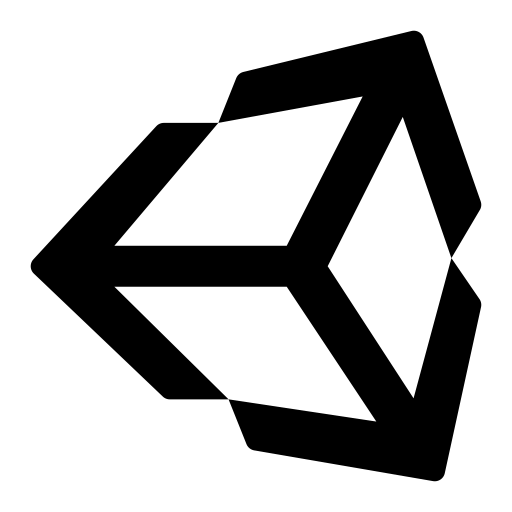
\includegraphics[width=\textwidth]{img/unity.png}
\end{minipage}
%
\section{Tecnologie Scelte}
%
\chapter{Sviluppo dell'Applicazione}
%
\section{Requisiti per l'Interfaccia Utente}
%
\section{Setup dell'Ambiente di Sviluppo}
%
\subsection{Librerie}
%
\section{Componenti}
%
\subsection{Raccoglitore di Dati}
%
\subsection{Calcolatore}
%
\subsection{Motore Grafico}
%
\chapter{Testing dell'Applicazione}
%
\section{Dati Utilizzati}
%
\section{Risultati Matematici}
%
\section{Risultato dell'Interfaccia Grafica}
%
\chapter{Commenti}
%
\chapter{Conclusioni}
%
\chapter{Ringraziamenti}
%
\chapter{Bibliografia}
%
\end{document}